% !TeX spellcheck = da_DK
\subsection{Spændingsforsyning} \label{Spaendingsforsying}
\subsubsection{Teori og design}
Til systemet anvendes to $1.5$V batterier som spændingsforsyning, der placeres i en spændingsregulator. Denne kan teoretisk levere en spænding på hhv. $\pm5.5$V og $\pm3.4$V fra to forskellige terminaler. Derudover besidder spændingsregulatoren en jordkobling, som øvrige komponenter i systemet kan kobles til. Til dette system benyttes begge terminaler; $\pm3.4$V forsyner med et input til referencespændingen til komparatoren, og $\pm5.5$V benyttes til resten af systemet. Spændingsregulatoren er designet således, at den leverer en spænding koblet i en split-supply. Spændingsregulatorens negative spændingsforsyninger kaldes $-V_{cc}$ og den positive kaldes $+V_{cc}$. \\%Den positive pol fra det ene batteri tilkobles den negative pol på det andet batteri i. Derudover dannes en fælles jordforbindelse for øvrige komponenter i systemet, som kræver en forbindelse til jord. Den negative pol i det første batteri i det første batteri anvendes som systemets negative forsyningsspænding og indikeres med $-V_{cc}$, mens det andet batteri anvendes som den positive spændingsforsyning og indikeres med $+V_{cc}$.
Da batterierne ikke leverer den samme spænding over hele batteriernes levetid, skal batteriet skiftes ud, når de ikke leverer den nødvendige spænding til systemet. Batteriernes levetid afhænger af, hvor meget strøm systemet trækker. %Da komparatorkonfigurationen kræver den højeste spænding iblandt blokkene, skal spændingsregulatoren minimum leverer en spænding på xx V. Derfor kræver systemt en minimal spænding på xx V.

\subsubsection{Simulering}
Ved simulering af spændingsforsyningen anvendes LTspice, hvor der sendes en spænding igennem en buffer, som også er beskrevet og benyttet i bilag \ref{Bilag:Pilotforsoeg} på side \pageref{Bilag:Pilotforsoeg}. Herved kan konsekvensen af et faldende input simuleres, således at kravet om at spændingsregulatorens forsyning ikke må forårsage klipning af signalet, kan undersøges. Det maksimale input, som vil blive indsendt igennem systemet uden der ønskes klipning af signalet, er $0.0037 \cdot 9.1 \cdot 3.6 25 = 3.030$V jævnført bilag \ref{Bilag:Pilotforsoeg} på side \pageref{Bilag:Pilotforsoeg}, hvorfor denne spænding benyttes i simuleringen som amplituden på et sinussignal. Konsekvensen af en faldende spændingsforsyning undersøges, hvilket er illustreret på \figref{fig:spaendingsforsyning_graf}. Der undersøges for hhv. $5.5$V, $5$V, $4.5$V og $4.0$V.
\begin{figure}[H]
	\centering
	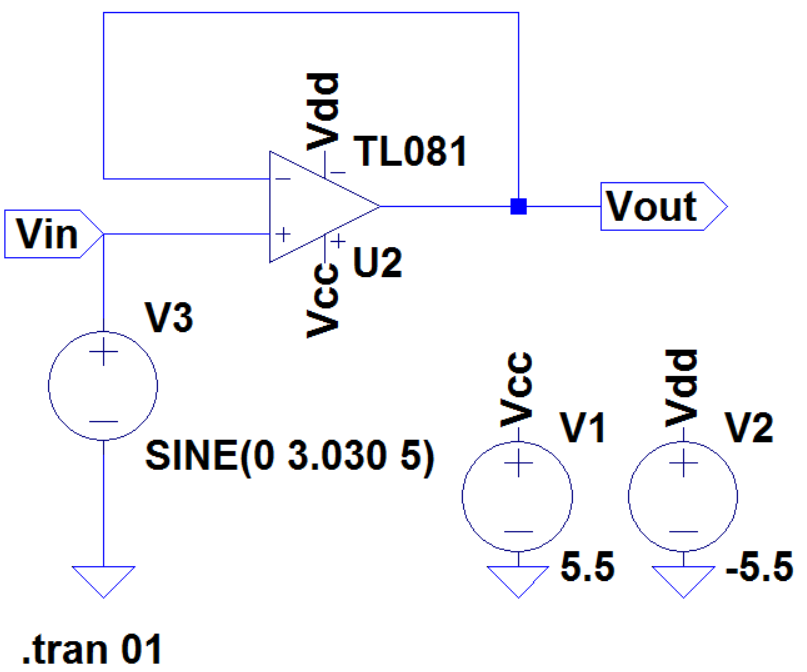
\includegraphics[scale=0.4]{figures/cProblemloesning/Spaendingsforsyning_LTspice2.PNG}
	\caption{På figuren ses designet af spændingsforsyningen med en buffer. Inputsignalet er en sinuskurve med en amplitude på det maksimalt ønskede signal i systemet. Spændingsforsyningen til operationsforstærkeren er på billedet $\pm5.5$V, hvilket er den spænding, som anvendes til at forsyne systemet.}
	\label{fig:spaendingsforsyning}
\end{figure}
\begin{figure}[H]
	\centering
	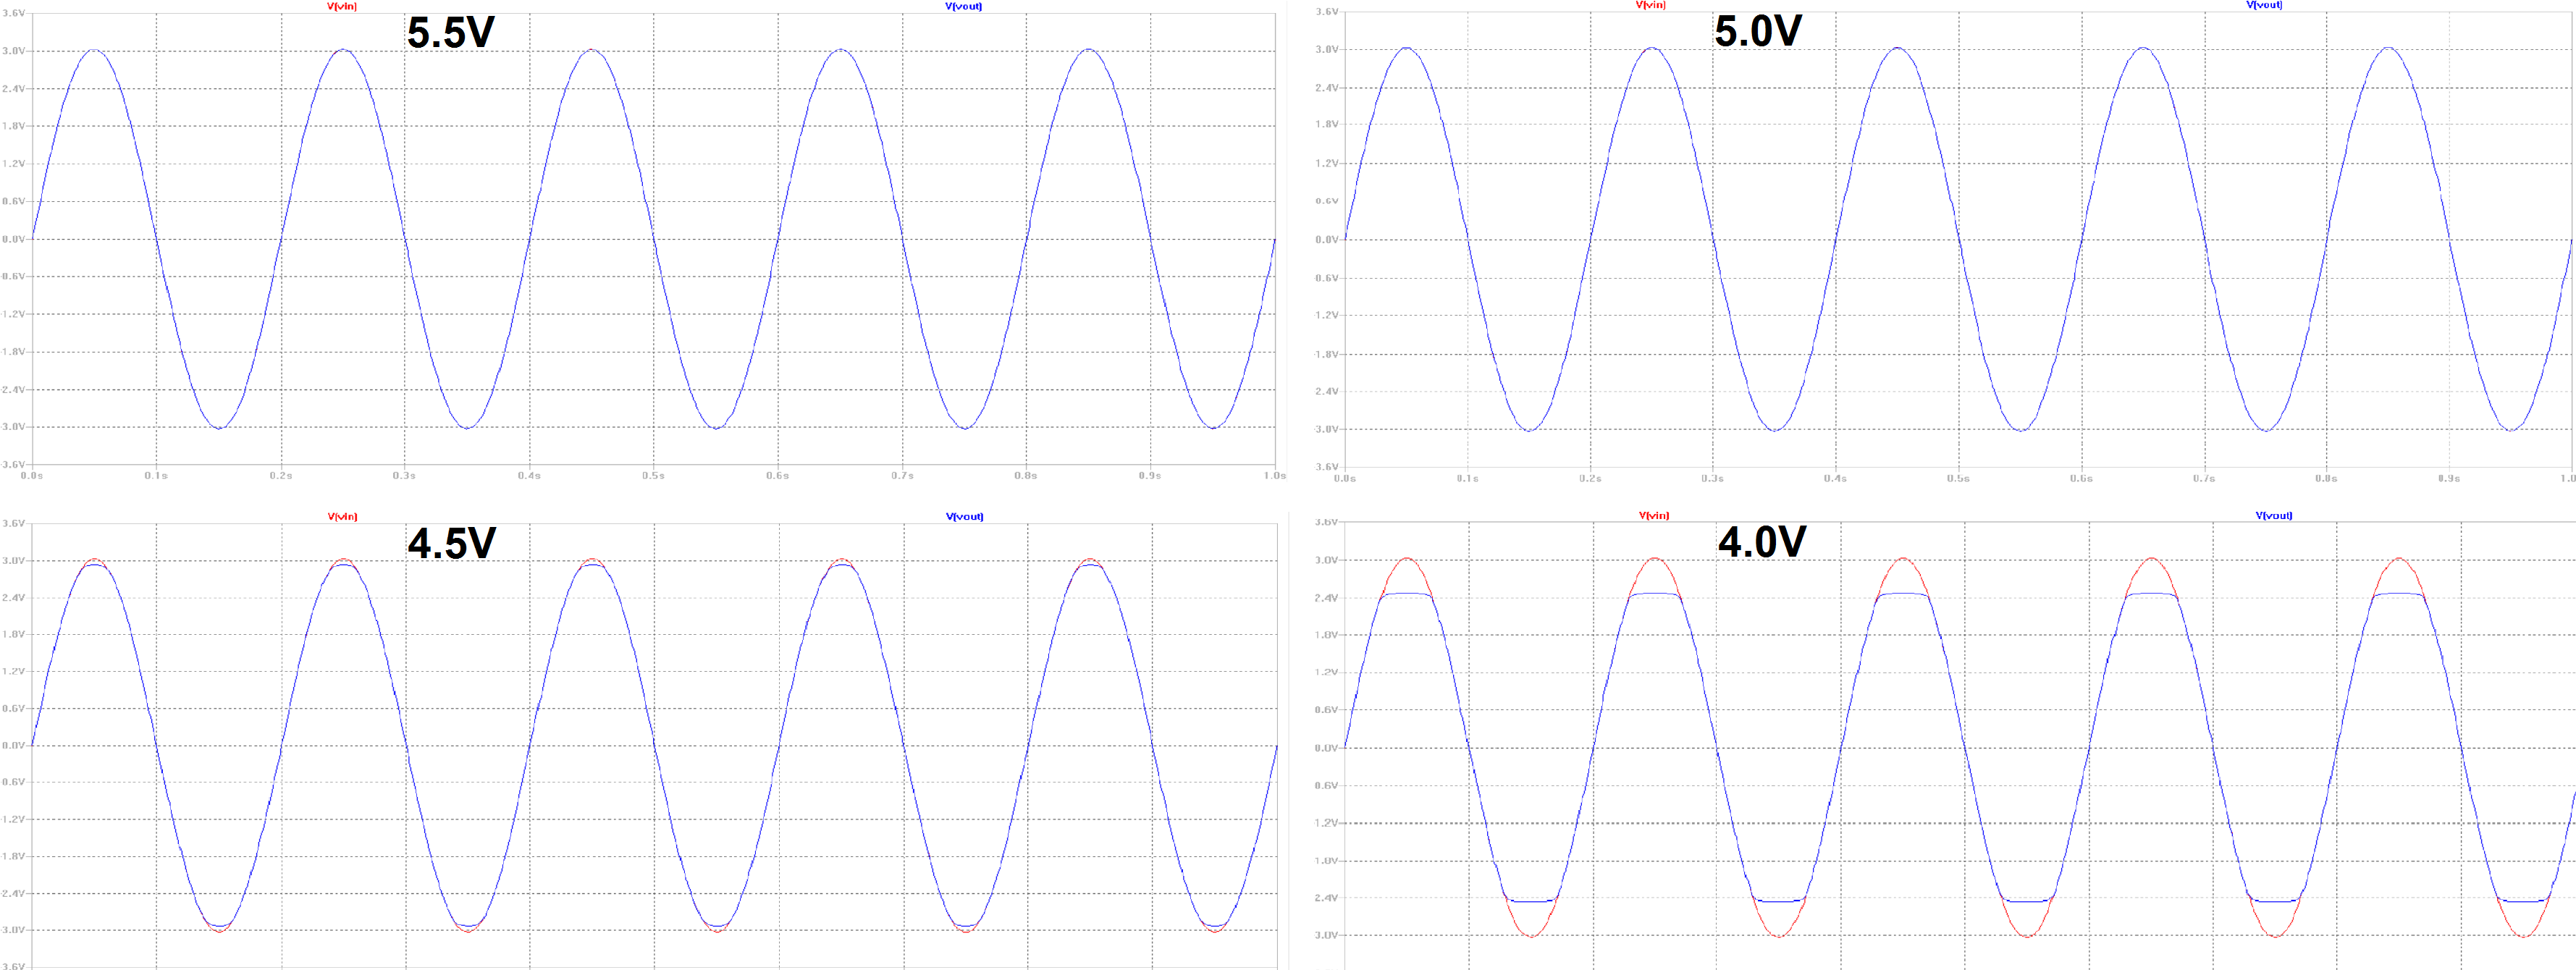
\includegraphics[scale=0.2]{figures/cProblemloesning/Spaendingsforsyning2.PNG}
	\caption{På figuren ses simuleringen af en spændingsforsyning på hhv. $5.5$V, $5$V, $4.5$V og $4.0$V for et inputsignal. Det fremgår af figuren, at signalet bliver klippet ved $4.5$V, hvilket ses tydeligere, når spændingsforsyningen bliver $4.0$V. Simulering er foretaget i LTspice.}
	\label{fig:spaendingsforsyning_graf}
\end{figure}
På \figref{fig:spaendingsforsyning_graf} ses simuleringen af systemet ved fire forskellige spændingsforsyninger. Der ses, at signalet ideelt vil blive klippet, hvis spændingsforsyningen leverer under $5.0$V til operationsforstærkerne.

\subsubsection{Implementering og test}
Det undersøges, hvorvidt spændingsregulatoren leverer en spænding på hhv. mindst $5.5$V samt $3.4$V fra hver terminal jævnfør afsnit \ref{Krav_spaending_spicifikt} på side \ref{Krav_spaending_spicifikt}. Derudover testes det, om spændingsregulatoren kan forsyne samtlige blokke i systemet med den minimalt krævede spænding samt forsyner operationsforstærkerne med mindst $5.0$V for at undgå klipning af signalet. \\
Batterierne blev inden testen målt til henholdsvis $1.5394$V og $1.5373$V. Ifølge afsnit \ref{Krav_spaending_spicifikt} på side \pageref{Krav_spaending_spicifikt} accepteres der ikke en spænding under $5.5$V, hvorimod der accepteres en afvigelse på $\pm10\%$ for $3.4$V. Derfor vil afvigelserne for spændingsforsyningen på $\pm5.5$V angives i V, hvorimod afvigelsen for $3.4$V angives i procent.
\begin{table}[H]
	\centering
	\begin{tabular}{|l|l|l|}
		\hline
		\textit{Teoretisk} & \textit{Målt} & \textit{Afvigelse} \\ \hline
		$\pm5.5$V          &     $5.5643$V \& -$5.5766$V   &     +$0.0643$V \& +$0.0766$V                 \\ \hline
		$3.4$V             &     $3.3746$V                 &      $0.75\%$                                \\ \hline
	\end{tabular}
	\caption{I tabellen ses outputtet fra spændingsregulatoren, når den ikke er koblet til det samlede kredsløb.}
	\label{tab:spaending_resultat}
\end{table}
 
\begin{table}[H]
	\centering
 	\begin{tabular}{l|l|l|l|}
 		\cline{2-4}                                                                                                                                      & \textit{Teoretisk} & \textit{Målt}                                                  & \textit{Afvigelse}                                              \\ \hline
 		\multicolumn{1}{|l|}{\textit{\begin{tabular}[c]{@{}l@{}}Spændingsforsyning\\ til accelerometer\end{tabular}}}                          & $\pm5.5$V          & $5.5315$V                                                      & $+0.0315$V                                                      \\ \hline
 		\multicolumn{1}{|l|}{\textit{\begin{tabular}[c]{@{}l@{}}Spændingsforsyning\\ til offsetjustering\end{tabular}}}                        & $\pm5.5$V          & \begin{tabular}[c]{@{}l@{}}$5.5386$V\\ -$5.5530$V\end{tabular} & \begin{tabular}[c]{@{}l@{}}+$0.0386$V\\ +$0.0530$V\end{tabular} \\ \hline
 		\multicolumn{1}{|l|}{\textit{\begin{tabular}[c]{@{}l@{}}Spændingsforsyning til \\ referencespænding til offsetjustering\end{tabular}}} & $\pm5.5$V          & \begin{tabular}[c]{@{}l@{}}$5.5384$V\\ -$5.5528$V\end{tabular} & \begin{tabular}[c]{@{}l@{}}+$0.0384$V\\ +$0.0528$V\end{tabular} \\ \hline
 		\multicolumn{1}{|l|}{\textit{\begin{tabular}[c]{@{}l@{}}Inputspænding til \\ referencespænding til offsetjustering\end{tabular}}}      & $\pm5.5$V          & $5.5320$V                                                      & +$0.0320$V                                                      \\ \hline
 		\multicolumn{1}{|l|}{\textit{\begin{tabular}[c]{@{}l@{}}Spændingsforsyning\\ til faktor $9.1$ forstærker\end{tabular}}}                & $\pm5.5$V          & \begin{tabular}[c]{@{}l@{}}$5.5308$V\\ -$5.5526$V\end{tabular} & \begin{tabular}[c]{@{}l@{}}+$0.0308$V\\ +$0.0526$V\end{tabular} \\ \hline
 		\multicolumn{1}{|l|}{\textit{\begin{tabular}[c]{@{}l@{}}Spændingsforsyning\\ til filter\end{tabular}}}                                 & $\pm5.5$V          & \begin{tabular}[c]{@{}l@{}}$5.5374$V\\ -$5.5292$V\end{tabular} & \begin{tabular}[c]{@{}l@{}}+$0.0374$V\\ +$0.0292$V \end{tabular} \\ \hline
 		\multicolumn{1}{|l|}{\textit{\begin{tabular}[c]{@{}l@{}}Spændingsforsyning\\ til faktor $3.6$ forstærker\end{tabular}}}                & $\pm5.5$V          & \begin{tabular}[c]{@{}l@{}}$5.5378$V\\ -$5.5293$V\end{tabular} & \begin{tabular}[c]{@{}l@{}}+$0.0378$V\\ +$0.0293$V\end{tabular} \\ \hline
 		\multicolumn{1}{|l|}{\textit{\begin{tabular}[c]{@{}l@{}}Spændingsforsyning til\\ komparatorblokken\end{tabular}}}                      & $\pm5.5$V          & \begin{tabular}[c]{@{}l@{}}$5.5358$V\\ -$5.5302$V\end{tabular} & \begin{tabular}[c]{@{}l@{}}+$0.0373$V\\ +$0.0302$V\end{tabular} \\ \hline
 		\multicolumn{1}{|l|}{\textit{\begin{tabular}[c]{@{}l@{}}Spændingsforsyning til \\ referencespænding til offsetjustering\end{tabular}}} & $\pm5.5$V          & \begin{tabular}[c]{@{}l@{}}$5.5373$V\\ $-5.5302$V\end{tabular} & \begin{tabular}[c]{@{}l@{}}+$0.0373$V\\ +$0.0302$V\end{tabular} \\ \hline
 		\multicolumn{1}{|l|}{\textit{\begin{tabular}[c]{@{}l@{}}Inputspænding til \\ referencespænding til komparatorblokken\end{tabular}}}    & $\pm5.5$V          & $5.5373$V                                                      & +$0.0373$V                                                      \\ \hline
 		\multicolumn{1}{|l|}{\textit{\begin{tabular}[c]{@{}l@{}}Spændingsforsyning til\\ vibratorer - før shothey diode\end{tabular}}}         & $3.4$V             & $3.3740$V                                                      & $0.76\%$                                                        \\ \hline
 	\end{tabular}
  	\caption{I tabellen ses forsyningen eller inputspænding blokkene i systemet.}
  	\label{tab:spaending_systemet}
\end{table}
I \tableref{tab:spaending_resultat} og \tableref{tab:spaending_systemet} ses det, at spændingsregulatoren har en afvigelse på $0.75\%$ ift. $3.4$V spændingen og leverer mindst $5.5$V, når spændingsregulatoren ikke er tilkoblet systemet. Efter tilkobling ses det i \tableref{tab:spaending_systemet}, at spændingsregulatoren forsyner blokkene i systemet med den minimale spænding, som er krævet for korrekt funktion. Det vides fra teorien og kan ses i simuleringen, at så længe spændingsforsyningen leverer mindst $5$V, vil den ikke forsage klipning af signalet. Hvis spændingen på teoretisk $3.4$V leverer under dette, vil det have en effekt på vibratorerne, da det kun er dem, som denne spænding benyttes til at forsyne. \\